\documentclass[aspectratio=169,xcolor=pdftex,dvipsnames,table]{beamer}\usepackage[]{graphicx}\usepackage[]{xcolor}
% maxwidth is the original width if it is less than linewidth
% otherwise use linewidth (to make sure the graphics do not exceed the margin)
\makeatletter
\def\maxwidth{ %
  \ifdim\Gin@nat@width>\linewidth
    \linewidth
  \else
    \Gin@nat@width
  \fi
}
\makeatother

\definecolor{fgcolor}{rgb}{0.345, 0.345, 0.345}
\newcommand{\hlnum}[1]{\textcolor[rgb]{0.686,0.059,0.569}{#1}}%
\newcommand{\hlsng}[1]{\textcolor[rgb]{0.192,0.494,0.8}{#1}}%
\newcommand{\hlcom}[1]{\textcolor[rgb]{0.678,0.584,0.686}{\textit{#1}}}%
\newcommand{\hlopt}[1]{\textcolor[rgb]{0,0,0}{#1}}%
\newcommand{\hldef}[1]{\textcolor[rgb]{0.345,0.345,0.345}{#1}}%
\newcommand{\hlkwa}[1]{\textcolor[rgb]{0.161,0.373,0.58}{\textbf{#1}}}%
\newcommand{\hlkwb}[1]{\textcolor[rgb]{0.69,0.353,0.396}{#1}}%
\newcommand{\hlkwc}[1]{\textcolor[rgb]{0.333,0.667,0.333}{#1}}%
\newcommand{\hlkwd}[1]{\textcolor[rgb]{0.737,0.353,0.396}{\textbf{#1}}}%
\let\hlipl\hlkwb

\usepackage{framed}
\makeatletter
\newenvironment{kframe}{%
 \def\at@end@of@kframe{}%
 \ifinner\ifhmode%
  \def\at@end@of@kframe{\end{minipage}}%
  \begin{minipage}{\columnwidth}%
 \fi\fi%
 \def\FrameCommand##1{\hskip\@totalleftmargin \hskip-\fboxsep
 \colorbox{shadecolor}{##1}\hskip-\fboxsep
     % There is no \\@totalrightmargin, so:
     \hskip-\linewidth \hskip-\@totalleftmargin \hskip\columnwidth}%
 \MakeFramed {\advance\hsize-\width
   \@totalleftmargin\z@ \linewidth\hsize
   \@setminipage}}%
 {\par\unskip\endMakeFramed%
 \at@end@of@kframe}
\makeatother

\definecolor{shadecolor}{rgb}{.97, .97, .97}
\definecolor{messagecolor}{rgb}{0, 0, 0}
\definecolor{warningcolor}{rgb}{1, 0, 1}
\definecolor{errorcolor}{rgb}{1, 0, 0}
\newenvironment{knitrout}{}{} % an empty environment to be redefined in TeX

\usepackage{alltt}
% \documentclass[notes,aspectratio=169,xcolor=pdftex,dvipsnames,table]{beamer}

%\setbeameroption{show notes}

\usepackage{bm,graphicx,amsmath,tikz} %fancybox,
\usepackage{color}%,textpos}
\usepackage[round]{natbib}
\usepackage[normalem]{ulem}
\usepackage{hyperref}
\usepackage{lastpage}
\usepackage{array}
\usepackage{color}
\usepackage{framed}

% Define Western colours
\definecolor{western}{rgb}{.306,.152,.524}
\definecolor{westerngray}{rgb}{.512,.508,.524}

%% Define BEAMER colours
\setbeamercolor{frametitle}{bg=western,fg=white}
\setbeamercolor{framesubtitle}{bg=western,fg=black}
\setbeamercolor{title}{fg=white,bg=western}
\setbeamercolor{author}{fg=white,bg=western}
\setbeamercolor{institute}{fg=white,bg=western}
\setbeamercolor{date}{fg=white,bg=western}

%% Set BEAMER fonts
\setbeamerfont{title}{shape=\bf}
\setbeamerfont{frametitle}{shape=\sc,size=\Large}
\setbeamerfont{framesubtitle}{shape=\sc,size=\Large}
\setbeamerfont{footline}{shape=\sc}

%% Define BEAMER toc
\setbeamercolor{section in toc}{fg=western}
\setbeamercolor{subsection in toc}{fg=westerngray}
\setbeamertemplate{sections/subsections in toc}[ball]

%% Define BEAMER background
\setbeamercolor{background canvas}{bg=white}

%% Define BEAMER footer
\setbeamertemplate{navigation symbols}{}
\setbeamercolor{footline}{fg=white,bg=western}
\setbeamertemplate{footline}{%
  \begin{beamercolorbox}[wd=\paperwidth]{footline}
    \vskip5pt

    \hspace{.1in}
    \raisebox{.05in}{
      \scriptsize{\bf \insertshorttitle }
    }
    \hfill
    \raisebox{.05in}{
      \scriptsize{\bf \insertframenumber/\pageref{LastPage}}
    }
    \hspace{5pt}

    \vskip5pt
  \end{beamercolorbox}
}

%% Define BLOCK environment
\setbeamercolor{block title}{fg=western}
\setbeamerfont{block title}{series=\bfseries}

%% Define ENUMERATE and ITEMIZE environements
\setbeamertemplate{itemize item}[ball]
\setbeamertemplate{enumerate item}[ball]
\setbeamercolor{item projected}{bg=western}

%% Define BEAMER toc
\setbeamercolor{sections/subsections in toc}{fg=blue!75}
\setbeamertemplate{sections/subsections in toc}[ball]

%% Define SECTION openings
\AtBeginSection[]{
}

\title[SS2857 -- Lecture 2]{SS2857 Probability and Statistics 1\\
  Fall 2024\\
  \vspace{.2in}
  Lecture 2}
  
\date{}




\IfFileExists{upquote.sty}{\usepackage{upquote}}{}
\begin{document}

{
\setbeamertemplate{footline}{}
\setbeamercolor{background canvas}{bg=western}

\begin{frame}
  \maketitle
\end{frame}
}


\begin{frame}
  \begin{center}
    \Large{\textbf{2.2 Axioms, Interpretations, and Properties of Probability}}

    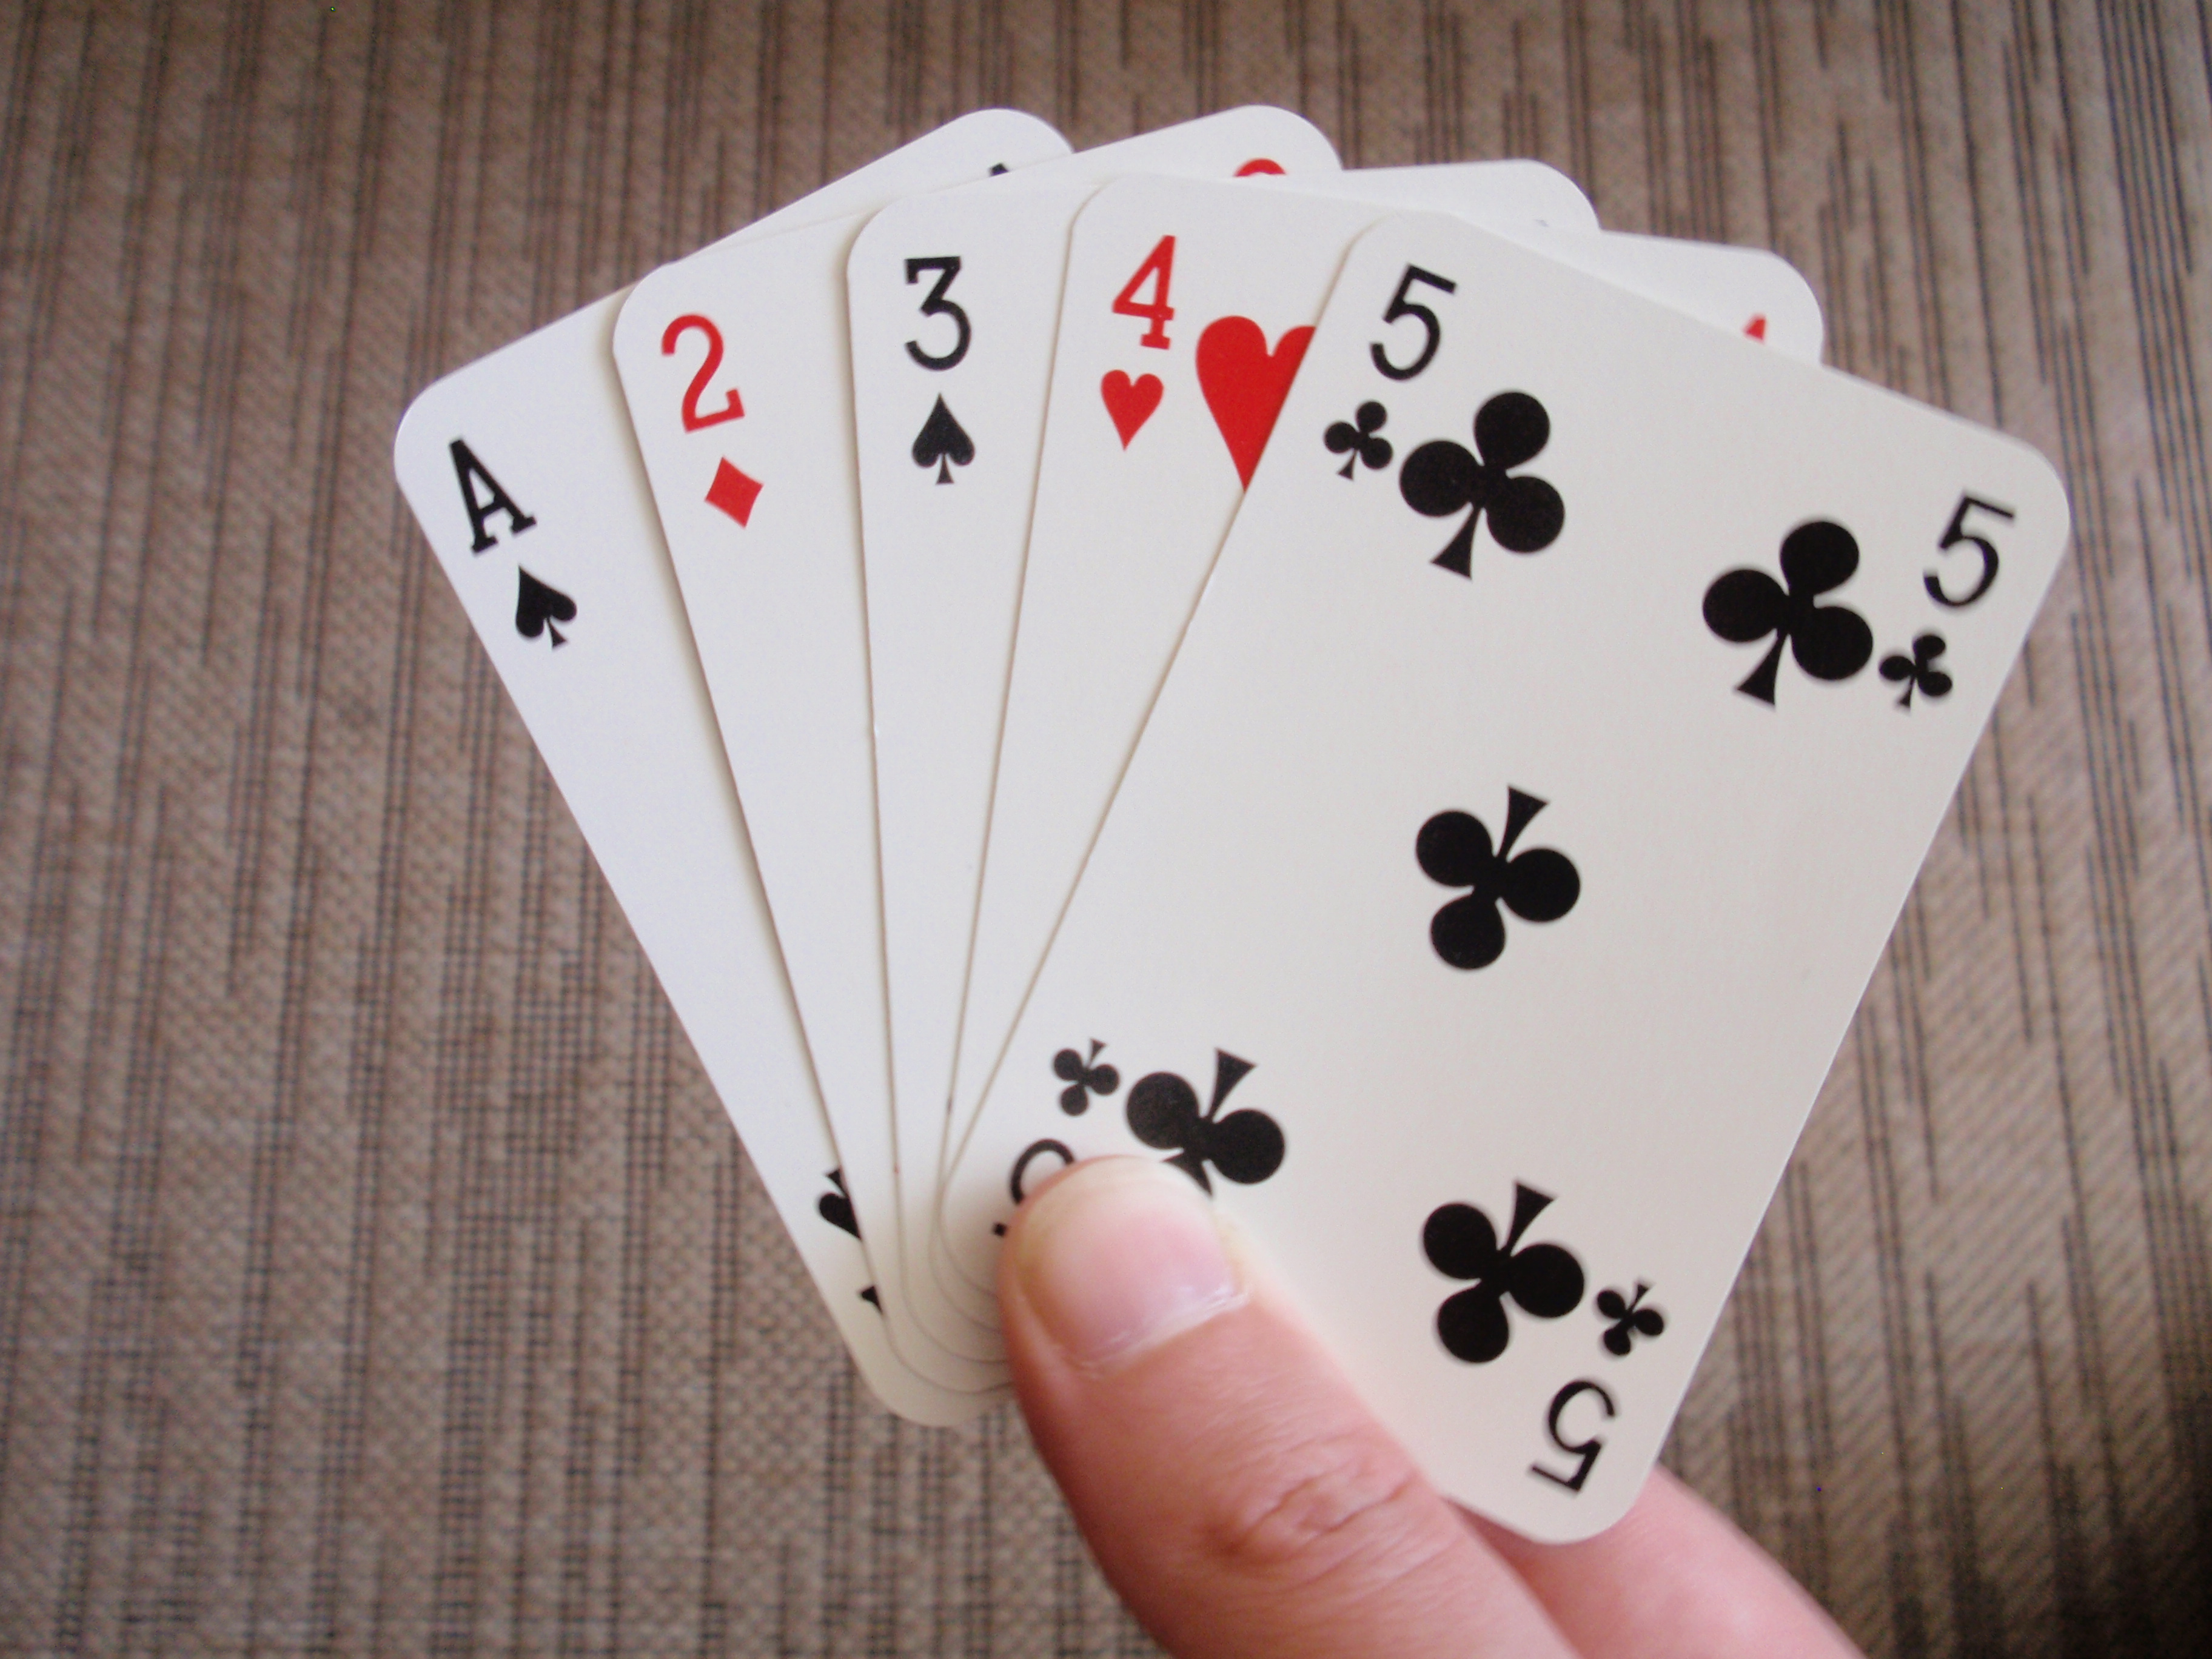
\includegraphics[height=.6\textheight]{Figures/AcetoFive}
  \end{center}
\end{frame}

\begin{frame}{Axioms of Probability}

  Let $\mathcal S$ be a samples space for some experiment. The three axioms of probability are:
  \begin{enumerate}
  \item The probability of any event is non-negative:
    \[
      P(A) \geq 0 \mbox{ for any } A \subset \mathcal S.
    \]
  \item The probability of the entire sample space is 1:
    \[
      P(\mathcal S)=1.
    \]

    %$A_1\cap A_2 \cap A_3 \cap \ldots = \cap_{i=1}^\infty A_i=\emptyset$
  \item The probability of an infinite union of disjoint events is the sum of the probabilities. 
  
  Given $A_1,A_2,A_3,\ldots \subset \mathcal{S}$ such that $A_i\cap A_j=\emptyset$ for every $i\neq j$
    \[
      P(A_1 \cup A_2 \cup A_3\ldots)=P(\cup_{i=1}^\infty A_i)=\sum_{i=1}^\infty P(A_i).
    \]
  \end{enumerate}
  
\end{frame}

\begin{frame}{Axioms of Probability}
  \begin{block}{Key Results 1}
    \begin{enumerate}
    \item Complement rule:
      \[
        P(A')=1-P(A).
      \]
    \item Probabilities are less than 1:
      \[P(A) \leq 1.\]
    \item Finite union of disjoint events:\\
      Given $A_1,A_2,A_3,\ldots,A_k \subset \mathcal{S}$ such that $A_i\cap A_j=\emptyset$ for every $i\neq j$ then
      \[
        P(A_1 \cup A_2 \cup A_3\ldots\cup A_k)=P(\cup_{i=1}^k A_i)=\sum_{i=1}^k P(A_i).
      \]
    \end{enumerate}
  \end{block}

\end{frame}

\begin{frame}{Axioms of Probability}
  \begin{block}{Key Results 2}
    \begin{enumerate}
     \item Union of two \textcolor{red}{events}:\\
      For any $A,B \subset \mathcal S$
      \[
        P(A \cup B)=P(A) + P(B) - P(A\cap B).
      \]
    \item Union of three \textcolor{red}{events}:\\
      For any $A,B,C \subset \mathcal S$
      \[
        P(A \cup B\cup C)=P(A) + P(B) +P(C) - P(A\cap B) -P(A\cap C) -P(B \cap C) + P(A \cap B \cap C).
      \]
      
    \end{enumerate}
  \end{block}

\end{frame}

\begin{frame}{Example 2.1}
  Suppose that the sample space, $\mathcal S$, contains $N>1$ outcomes and we assign each event $A \subset \mathcal S$ probability
  \[
    P(A)=\left(\frac{N(A)}{N}\right)^k
  \]
  where $N(A)$ denotes the number of outcomes in $A$ for some positive integer $k$, i.e. $k \in \mathbb{Z}^+$.

  \medskip

  \begin{center}
    For what values of $k$ is this assignment valid?
  \end{center}
  
\end{frame}

\begin{frame}{Equally Likely Outcomes}

  If all outcomes in the sample space are equally likely, then 
\begin{enumerate}  
  \item the probability of any simple event (outcome) is $1/N$, 
  \item the probability of any event $A$ is
  \[
    P(A)=\frac{N(A)}{A}.
  \]
  \end{enumerate}
  
\end{frame}

\begin{frame}{Example 2.2}
  \begin{block}{Happy Birthmonth!}
    Consider the events $E_1$, $E_2$, and $E_3$ from Example 1.1 part 2. 
    \medskip

    \begin{itemize}
    \item $E_1=A_1 \bigcap B_1 \bigcap C_1$
    \item $E_2=\bigcup_{i=1}^{12} (A_i \bigcap B_i \bigcap C_i)$
    \item $E_3=\bigcup_{i=1}^{12} (A_i \bigcap B_i \bigcap C_i')$
    \end{itemize}

    \medskip
    Suppose that the probability of any outcome is equally likely. 
    \begin{enumerate}[a)]
    \item What is the probability of each event?
    \item What is the probability that exactly 2 of the students are born in the same month?
    \item What is the probability that at least 2 of the students are born in the same month?
    \item What does the probability in part c) mean?
    \end{enumerate}
  \end{block}
\end{frame}

\begin{frame}{Interpreting Probability}

  \begin{block}{Definition}
    Suppose that we repeat the same experiment $n$ times. The probability of an event $A$ is the \textit{limiting relative frequency} of the event as $n \to \infty$:
    \[
      P(A)=\lim_{n \to \infty} \frac{n(A)}{n}.
    \]

    \bigskip

    \begin{center}
      If we repeat the same experiment many, many times then the proportion of times we observe the event $A$ will be very close to $P(A)$ and get closer and closer as the number of replicates increases. 
    \end{center}
    
  \end{block}
\end{frame}

\begin{frame}{Example 2.3}
  Provide an interpretation for the following statements:
  \begin{enumerate}
  \item The probability that a randomly selected number between 1 and 10 is prime is $.5$.
  \item The probability that we draw a club from a well shuffled deck of cards is $.25$.
  \item The probability that a randomly selected newborn baby is assigned to be male at birth is $.503$. 
  \item The probability that it will rain this afternoon is $.70$.
  \end{enumerate}
\end{frame}

\begin{frame}{Exercise 2.1}

You and your friend play a game of chance. They think of a number between 1 and 10, and you try to guess it. You win if you guess the number. 

Suppose that your friend choose the number at random (i.e., the numbers are equally likely). 

\begin{enumerate}[a)]
\item Compute the probability of winning and provide an interpretation.
\item What is the probability that your guess is exactly one number away from the number your friend chose?
\item What is the probability that your guess is within one number of the number your friend chose?
\item What is the probability that your guess is more than one number away from the number your friend chose?
\end{enumerate}
\end{frame}

\begin{frame}
  \begin{center}
    \Large{\textbf{Questions?}}
  \end{center}
\end{frame}

\end{document}
